\chapter{Game Design}
The game that will be analysed is called "Space-run" and it involves attempting to accumulate the highest score possible by navigating through three distinct tunnels while avoiding various obstacles. The game is endless in nature, as the speed increases each time the player successfully completes all three tunnels.

\section{Player and Movement}
In "Space-run" the player assumes control of a character named Hans, who is responsible for dodging obstacles by moving left and right. In addition to these lateral movements, Hans also has the ability to shoot bullets and defeat certain in-game creatures, which results in a higher score. The player must utilize these abilities in order to progress through the game and achieve a high score.

\section{Obstacles}
As previously stated, the player must navigate through various obstacles in the game. These obstacles can be divided into three distinct categories, and each tunnel contains a unique subset of them. In the subsequent sections, we will delve deeper into these categories in order to better understand the challenges faced by the player.

\subsection{Traps}
\begin{figure}[h]
    \centering
    
\includegraphics[width=\textwidth]{traps}
    \caption{Trap examples}
    \label{fig:mesh1}
\end{figure}
As depicted in Figure \ref{fig:mesh1}, a selection of the various trap types that the character Hans must avoid is presented. These traps, of which there are a total of 10, vary in their level of difficulty and can be either static or animated. These traps can be encountered in any of the three tunnels, and if the player fails to successfully evade them, they result in an instant death.

\subsection{Bugs}
\label{Bugs}
\begin{figure}[h]
    \centering
    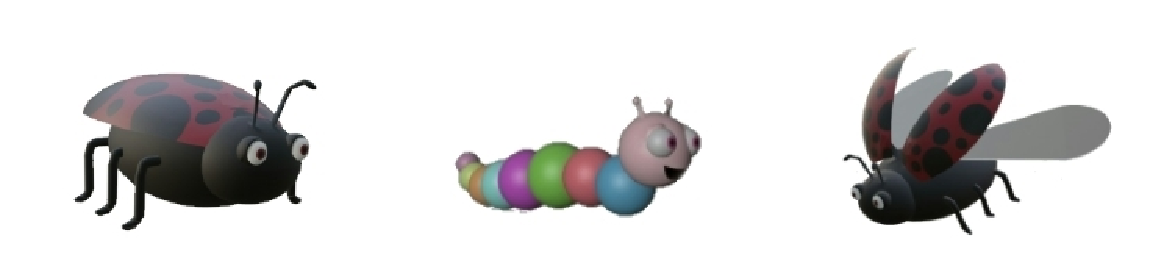
\includegraphics[width=\textwidth]{bugs}
    \caption{Bugs}
    \label{fig:mesh2}
\end{figure}
In addition to traps, the game also features bugs as an obstacle (as shown in Figure \ref{fig:mesh2}). These bugs typically appear in the second tunnel and are designed to align with the player, making them more challenging to evade. However, they can still be avoided by the player. If the player chooses to engage with the bugs, they can be defeated by shooting three bullets at them. If the player collides with a bug, Hans will lose 25\% of his battery life(for more information on battery life, see Section \ref{AdditionalFeatures}).

\subsection{Viruses}
	\begin{figure}[h]
    \centering
    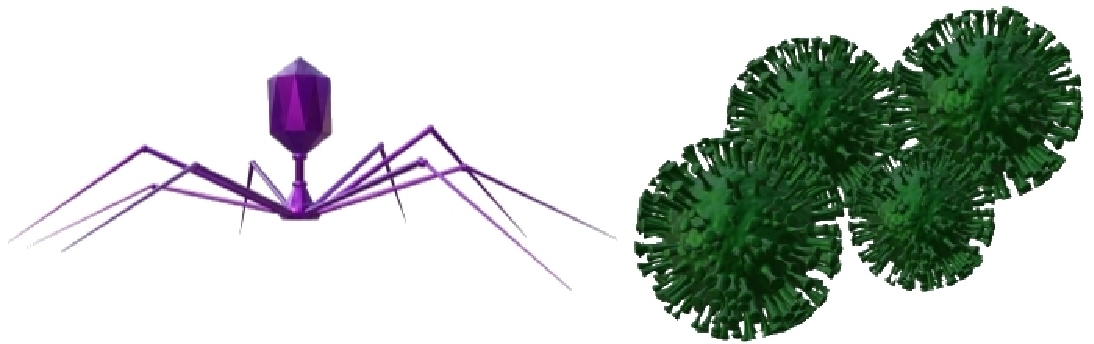
\includegraphics[width=\textwidth]{viruses}
    \caption{Bacteriophage and Rotavirus}
    \label{fig:mesh3}
\end{figure}
The third and final type of obstacle in the game are viruses (illustrated in Figure \ref{fig:mesh3}). These viruses are typically found in the third tunnel and, like bugs, can be eliminated through the use of three bullets. They also align with the player's movement, making them more difficult to evade, although it is still possible to do so. Bacteriophage, a subtype of virus, will result in an instant death if the player comes into contact with them. Rotaviruses, on the other hand, will cause the player's character to become sick for a brief period of time. During this illness, it is crucial for the player to avoid coming into contact with another Rotavirus, as this will result in the end of the game.

\section{Additional Features}
\label{AdditionalFeatures}
There are several other features of the game that are worth mentioning. One of the most significant of these is the battery life of the player's character, Hans, which is displayed on the right side of the screen. As Hans is designed to resemble a computer, it is necessary for him to recharge his battery throughout the game by collecting energy tokens. This will fully restore his battery capacity. There are three main ways in which Hans can lose battery life: running causes a constant reduction of 1\%, each bullet shot costs 1\% of the battery life, and coming into contact with a bug results in a reduction of 25\% (as described in Section \ref{Bugs}). If the battery reaches 0\%, Hans will die and the game will end.

Finally, it should be noted that upon successfully navigating through all three types of tunnels, the game will increase in speed and the player will once again encounter the same tunnels, looping through them indefinitely until the player loses.

\section{Score Count and Winning}
The score of the game is based on the length of time that the player is able to survive. Additionally, each time a player successfully shoots down a bug or virus, their score increases by 10 points. As previously mentioned, the game is designed to be played indefinitely, but for the purpose of this study, we have set the game to be considered won after an agent successfully completes nine tunnels, reaching level 10.
